\documentclass[a4paper, 12pt]{report}
\usepackage{graphicx}
\usepackage{xspace}
\usepackage[margin= 1in,includefoot]{geometry}
\newcommand\nth{\textsuperscript{th}\xspace}
\usepackage{xcolor}
\usepackage{lipsum}
\usepackage{listings}
\begin{document}
\begin{figure}
\includegraphics[scale=.63]{medipol.png}
\centering
\end{figure}
\begin{titlepage}
\title{Fall 2021, Computer Vision \\ Homework 1}
\author{by 64160010 - Rumeysa ÇELİK}
\maketitle
\end{titlepage}
\section*{{\textbf{Problem Set 1}}}
\textbf{Problem 1:} (Basic image operations)
\\ \\
\begin{figure}[h]
\includegraphics[scale=.39]{huser.jpeg}
\centering
\caption{Input Image}
\end{figure}
\\ \\ \\
A Python script was written to crop a region from the center; region size set to be half the size of the input image. Image saved as png file. The red channel of the image was extracted and displayed. The image has been converted to grayscale and displayed. Sobel filters in the x and y directions were defined in the code. These filters were applied to the grayscale image and the results were displayed. Gradient magnitude and gradient direction were obtained using these gradients. Found a way to show gradient direction; The gradient magnitude and gradient direction are displayed. Laplacian of Gaussian images were obtained for different sigma values and the results were displayed. \\ \\ \\
\textbf{Code:}

\definecolor{codegreen}{rgb}{0,0.6,0}
\definecolor{codegray}{rgb}{0.5,0.5,0.5}
\definecolor{codepurple}{rgb}{0.58,0,0.82}
\definecolor{backcolour}{rgb}{0.95,0.95,0.92}

\lstdefinestyle{mystyle}{
    backgroundcolor=\color{backcolour},   
    commentstyle=\color{codegreen},
    keywordstyle=\color{magenta},
    numberstyle=\tiny\color{codegray},
    stringstyle=\color{codepurple},
    basicstyle=\ttfamily\footnotesize,
    breakatwhitespace=false,         
    breaklines=true,                 
    captionpos=b,                    
    keepspaces=true,                 
    numbers=left,                    
    numbersep=5pt,                  
    showspaces=false,                
    showstringspaces=false,
    showtabs=false,                  
    tabsize=2
}

\lstset{style=mystyle}
\begin{lstlisting}[language=Python]
# -*- coding: utf-8 -*-
"""
Created on Fri Oct 31 19:11:12 2021

@author: Rumeysa CELIK
"""
from PIL import Image
import cv2
import matplotlib.pyplot as plt
import numpy as np


#PART A: Write a Python scriptto crop out a region from the center; the region size      should be half the size of the input image. Save the image as a pngfile.

img= cv2.imread("/Users/rumeysacelik/Desktop/ComputerVisionHW1/huser.jpeg",cv2.COLOR_BGR2GRAY)

cv2.imshow('original image',img)

print("ORIGINAL IMAGE SHAPE:",img.shape) # Print image shape
#Cropping an image

width, height = img.shape[1], img.shape[0]
c_x,c_y=int(width/2),int(height/2) 
mid_x, mid_y = int(width/2), int(height/2)


cropped_img = img[c_y-int(c_y/2):c_y+int(c_y/2),c_x-int(c_x/2):c_x+int(c_x/2)]
print("CROPPED IMAGE SHAPE:",cropped_img.shape)  

# Display cropped image
cv2.imshow("cropped image", cropped_img)

# Save the cropped image
cv2.imwrite("output/Cropped_Image.png", cropped_img)



#PART B: Extract the red channelof the imageand display it.

red_img= img[:,:,2]
cv2.imshow("RED_image", red_img)
# Save the red image
cv2.imwrite("output/RED_image.png", red_img)
 

#PART C: Convert the image to grayscaleand display it.

gray_img= cv2.cvtColor(img, cv2.COLOR_BGR2GRAY) #converts BGR to gray
cv2.imshow('GRAY_img',gray_img)
# Save the red image
cv2.imwrite("output/GRAY_img.png", gray_img)

#PART D: Define the Sobel filters in x and y directionsin your code. Apply thesefilters to the grayscale image and displaythe results.Using these gradients, obtain the gradient magnitude and gradient orientation. Find out a way to display the gradient orientation; display the gradient magnitude and gradient orientation.


gX = cv2.Sobel(gray_img, ddepth=cv2.CV_64F, dx=1, dy=0, ksize=5)
gY = cv2.Sobel(gray_img, ddepth=cv2.CV_64F, dx=0, dy=1, ksize=5)

 # scaling the gradients
gX = cv2.convertScaleAbs(gX)
gY = cv2.convertScaleAbs(gY)


# combining the gradient representations into a single image with addWeighted by giving them equal weight
combined = cv2.addWeighted(gX, 0.5, gY, 0.5, 0)
# show our output images
cv2.imshow("Sobel_X", gX)
cv2.imshow("Sobel_Y", gY)
cv2.imshow("Sobel_Combined", combined)
# Save the sobel images
cv2.imwrite("output/Sobel_X.png", gX)
cv2.imwrite("output/Sobel_Y.png", gY)
cv2.imwrite("output/Sobel_Combined.png", combined)

# computing the gradient magnitude and orientation
magnitude = np.sqrt((gX ** 2) + (gY ** 2))
orientation = np.arctan2(gY, gX) * (180 / np.pi) % 180 #converting to degree


print("MAGNITUDE\n",magnitude)
print("ORIENTATION\n",orientation)

#converting the arrays from float16 to uint8 to display
magnitude =magnitude.astype(np.uint8)
orientation =orientation.astype(np.uint8)

print("MAGNITUDE\n",magnitude)
print("ORIENTATION\n",orientation)
# Save the gradient magnitude and orientation 
cv2.imwrite("output/magnitude.png", magnitude)
cv2.imwrite("output/orientation.png", orientation)


# initializing a [1,3] figure to display the input grayscale image along with
# the gradient magnitude and orientation representations, respectively
(fig, axs) = plt.subplots(nrows=1, ncols=3, figsize=(16, 12))
# plot each of the images
axs[0].imshow(gray_img, cmap="gray")
axs[1].imshow(magnitude, cmap="jet")
axs[2].imshow(orientation, cmap="jet")
# set the titles of each axes
axs[0].set_title("Grayscale")
axs[1].set_title("Gradient Magnitude")
axs[2].set_title("Gradient Orientation [0, 180]")
# loop over each of the axes and turn off the x and y ticks
for i in range(0, 3):
	axs[i].get_xaxis().set_ticks([])
	axs[i].get_yaxis().set_ticks([])
# show the plots
plt.tight_layout()
plt.savefig('/Users/rumeysacelik/Desktop/ComputerVisionHW1/gradient.png')
plt.show()

#PART E: Obtain Laplacian of Gaussian imagefor different sigma values, and displaythe results.

"""Laplacian of Gaussian (LoG) is same as applying gaussian smooothing filter first and then 
computing laplacian of the result"""
# Removing noise by blurring with a Gaussian filter
sigma=0####"
src = cv2.GaussianBlur(img, (3, 3),sigma)
# Converting the image to grayscale
src_gray = cv2.cvtColor(src, cv2.COLOR_BGR2GRAY)
# [laplacian]
# Applying Laplace function
dst = cv2.Laplacian(src_gray, cv2.CV_16S, ksize=3)
# converting back to uint8
log = cv2.convertScaleAbs(dst)
# Save the log image
cv2.imwrite("output/Laplacian of Gaussian(sigma=0).png", log)

cv2.imshow("Laplace of Gaussian-sigma=0", log)


sigma=15####
# Removing noise by blurring with a Gaussian filter
src = cv2.GaussianBlur(img, (3, 3),sigma)
# Converting the image to grayscale
src_gray = cv2.cvtColor(src, cv2.COLOR_BGR2GRAY)
# [laplacian]
# Applying Laplace function
dst = cv2.Laplacian(src_gray, cv2.CV_16S, ksize=3)
# converting back to uint8
log = cv2.convertScaleAbs(dst)
# Save the log image
cv2.imwrite("output/Laplacian of Gaussian(sigma=15).png", log)

cv2.imshow("Laplace of Gaussian-sigma=15", log)

cv2.waitKey(0)
cv2.destroyAllWindows()

\end{lstlisting}
\newpage
\textbf{All outputs:}
\\
\begin{figure}[h]
\includegraphics[scale=.39]{1.png}
\centering
\end{figure}
\begin{figure}
\includegraphics[scale=.39]{2.png}
\centering
\end{figure}
\begin{figure}
\includegraphics[scale=.39]{3.png}
\centering
\end{figure}
\begin{figure}
\includegraphics[scale=.39]{4.png}
\centering
\end{figure}
\begin{figure}
\includegraphics[scale=.39]{5.png}
\centering
\end{figure}
\begin{figure}
\includegraphics[scale=.39]{6.png}
\centering
\end{figure}
\begin{figure}
\includegraphics[scale=.39]{7.png}
\centering
\end{figure}
\begin{figure}
\includegraphics[scale=.39]{8.png}
\centering
\end{figure}
\begin{figure}
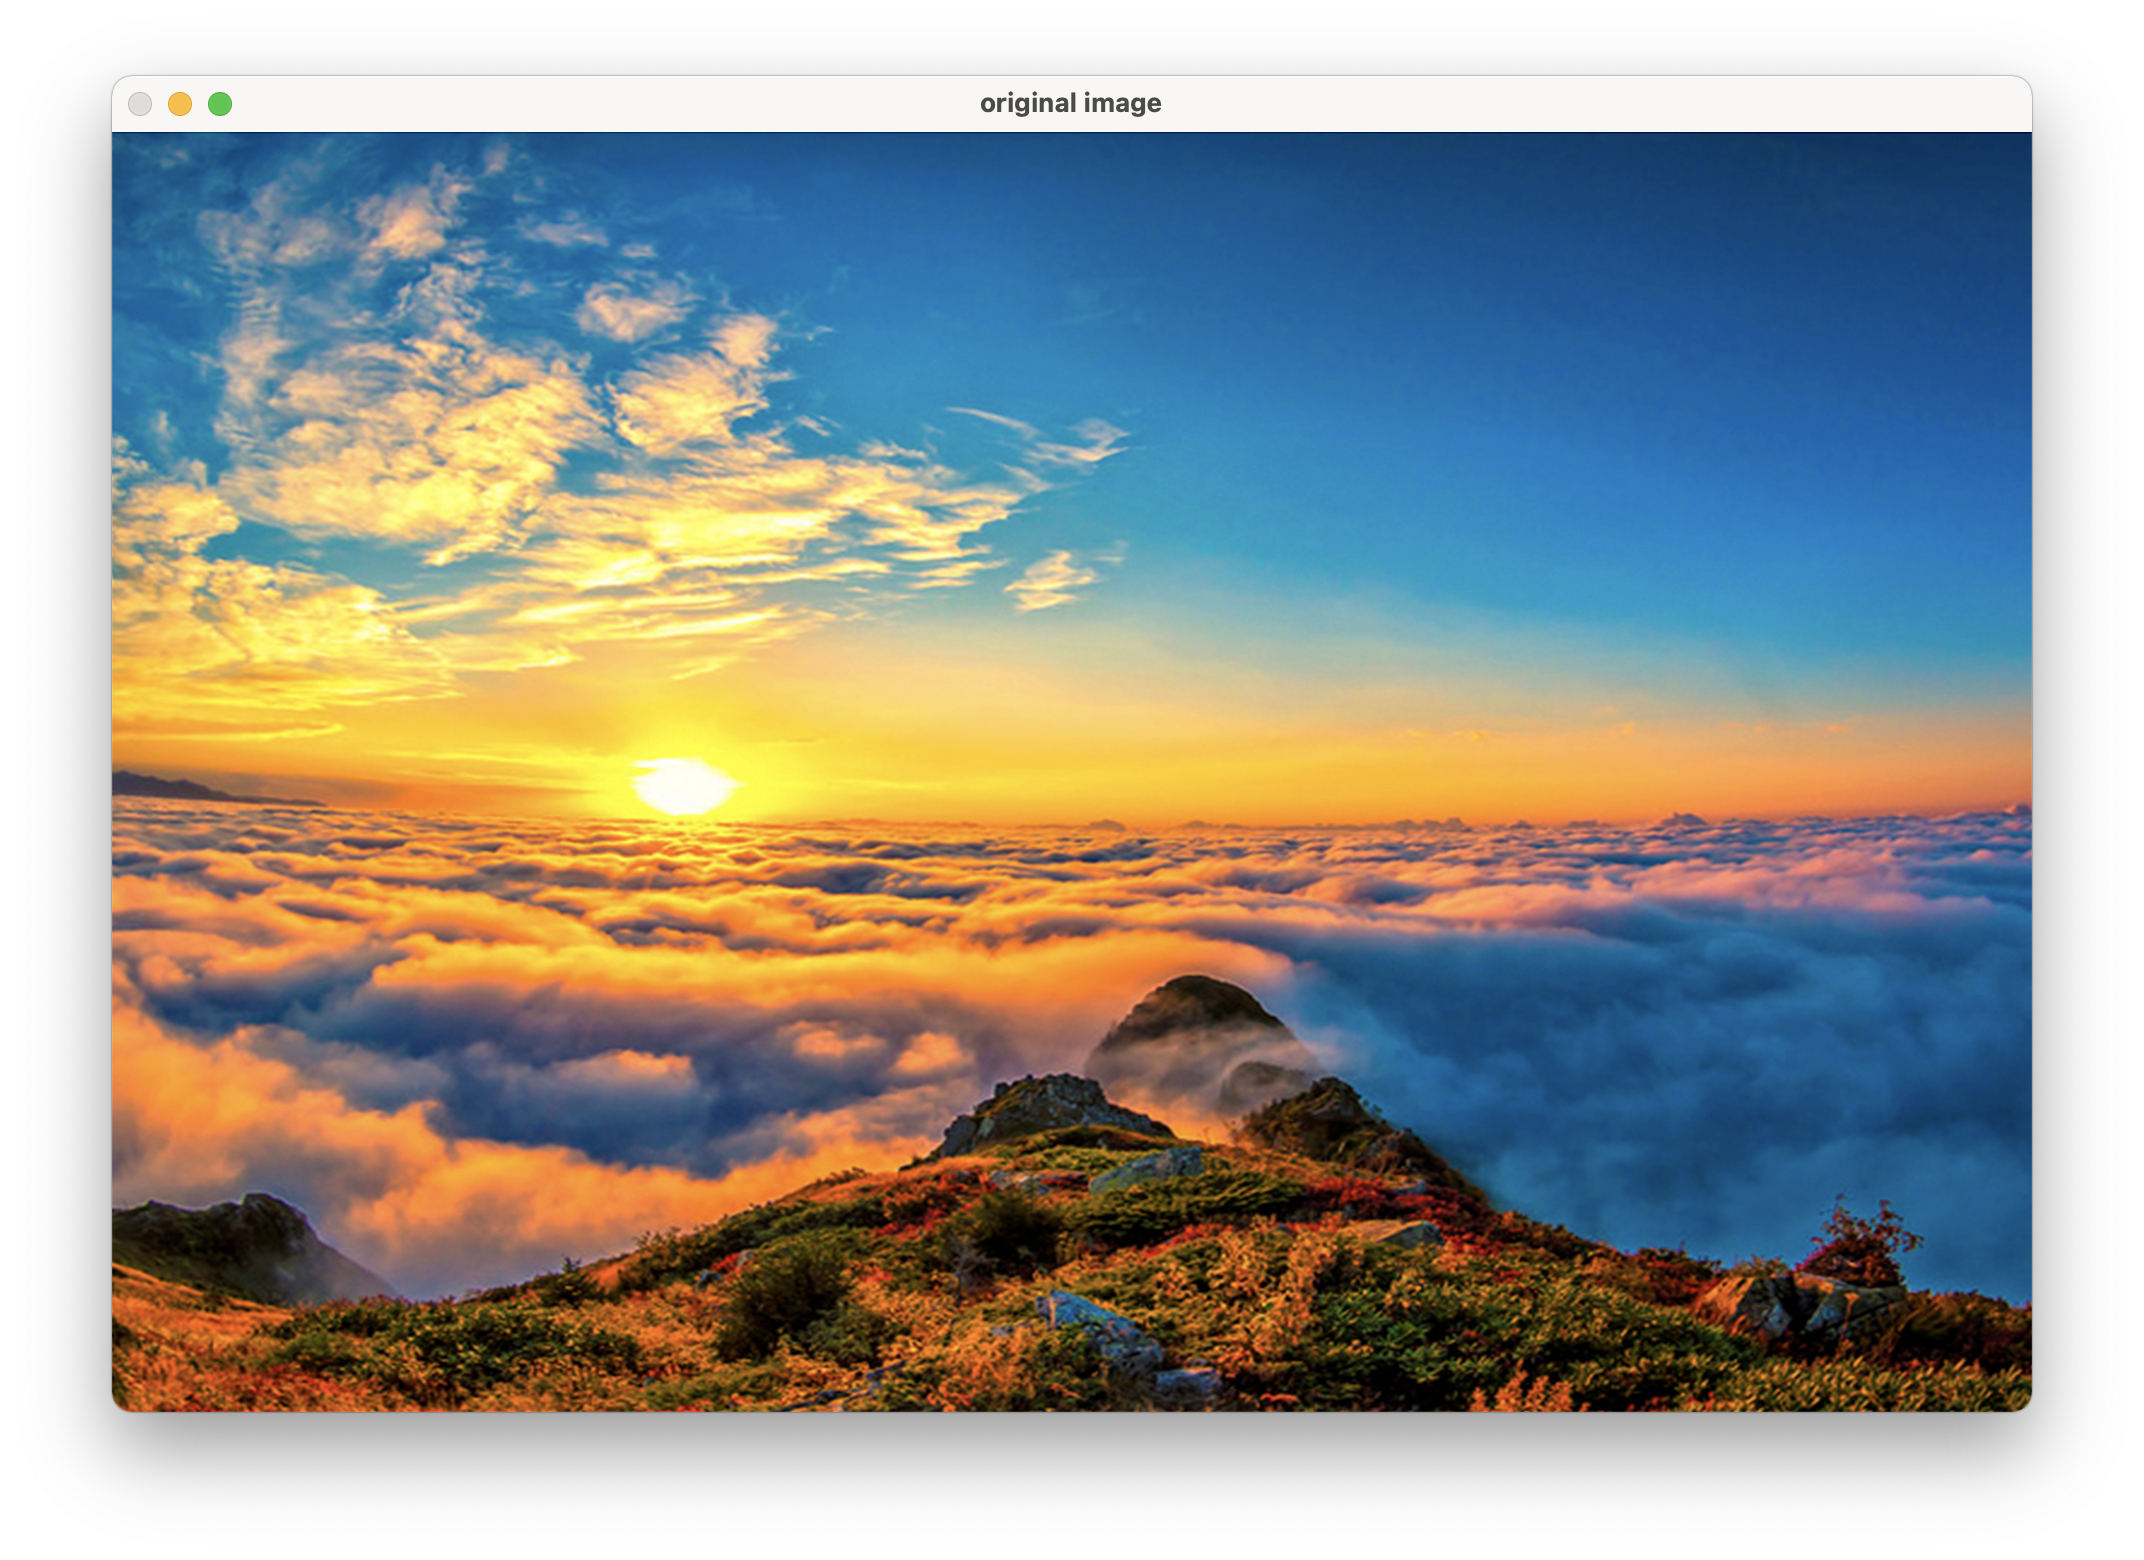
\includegraphics[scale=.39]{9.png}
\centering
\end{figure}
\begin{figure}
\includegraphics[scale=.39]{gradient.png}
\centering
\end{figure}
\begin{figure}
\includegraphics[scale=.43]{10.png}
\centering
\end{figure}
\newpage
\textbf{Problem 2:} (Basic video operations)
\\ \\
A Python script was written to receive a live video stream from the computer's webcam, the gradient size was calculated on the grayscale version of the image, and its input and gradient size displayed on the screen.
\\ \\ \\
\textbf{Code:}
\definecolor{codegreen}{rgb}{0,0.6,0}
\definecolor{codegray}{rgb}{0.5,0.5,0.5}
\definecolor{codepurple}{rgb}{0.58,0,0.82}
\definecolor{backcolour}{rgb}{0.95,0.95,0.92}

\lstdefinestyle{mystyle}{
    backgroundcolor=\color{backcolour},   
    commentstyle=\color{codegreen},
    keywordstyle=\color{magenta},
    numberstyle=\tiny\color{codegray},
    stringstyle=\color{codepurple},
    basicstyle=\ttfamily\footnotesize,
    breakatwhitespace=false,         
    breaklines=true,                 
    captionpos=b,                    
    keepspaces=true,                 
    numbers=left,                    
    numbersep=5pt,                  
    showspaces=false,                
    showstringspaces=false,
    showtabs=false,                  
    tabsize=2
}

\lstset{style=mystyle}
\begin{lstlisting}[language=Python]
# -*- coding: utf-8 -*-
"""
Created on Fri Oct 31 19:11:12 2021

@author: Rumeysa CELIK
"""
# -*- coding: utf-8 -*-
"""
Created on Sat Nov 1 01:54:05 2021

@author: Rumeysa CELIK
"""
import cv2
import numpy as np
import time 

#PART A: Write a Python script to take live video stream from the webcam of your computer, compute the gradient magnitude on the grayscale version of the image, and display the input and the gradient magnitude on the screen. 


# define a video capture object
vid = cv2.VideoCapture(0)
# used to record the time when we processed last frame
prev_frame_time = 0

# used to record the time at which we processed current frame
new_frame_time = 0

# font which we will be using to display FPS
font = cv2.FONT_HERSHEY_SIMPLEX

while True:
      
    # Capture the video frame by frame
    ret, frame = vid.read()
    
    # Display the resulting frame
    # putting the FPS count on the frame
 
    # time when we finish processing for this frame
    new_frame_time = time.time()
    # Calculating the fps
    
    # fps will be number of frame processed in given time frame
    # since their will be most of time error of 0.001 second
    # we will be subtracting it to get more accurate result
    fps = 1/(new_frame_time-prev_frame_time)
    prev_frame_time = new_frame_time
       
    # converting the fps into integer
    fps = int(fps)
       
    # converting the fps to string so that we can display it on frame
       	# by using putText function
    fps = str(fps)
    cv2.putText(frame, "FPS:"+fps, (7, 70), font, 3, (100, 255, 0), 3, cv2.LINE_AA)
    cv2.imshow('frame', frame)
    

    # # Convert to grayscale
    gray = cv2.cvtColor(frame, cv2.COLOR_BGR2GRAY) #converts BGR to gray
   
    
    # # Apply sobel filter in x and y directions
    grad_x = cv2.Sobel(gray,cv2.CV_64F,1,0,ksize=5) #x gradient
    grad_y = cv2.Sobel(gray,cv2.CV_64F,0,1,ksize=5) #y gradient
    


    # # scale the gradient to -1 to 1 range
    grad_x = grad_x / np.absolute(grad_x).max()
    grad_x = np.uint8(128+127*grad_x)
    grad_y = grad_y / np.absolute(grad_y).max()
    grad_y = np.uint8(128+127*grad_y)

  
    # computing the gradient magnitude and orientation
    magnitude = np.sqrt((grad_x ** 2) + (grad_y ** 2))
    orientation = np.arctan2(grad_y, grad_x) * (180 / np.pi) % 180 #converting to degree
    
    #converting the arrays from float16 to uint8 to display
    magnitude =magnitude.astype(np.uint8)
    orientation =orientation.astype(np.uint8)
    
    # time when we finish processing for this frame
    new_frame_time = time.time()
    # Calculating the fps
    
    # fps will be number of frame processed in given time frame
    # since their will be most of time error of 0.001 second
    # we will be subtracting it to get more accurate result
    fps = 1/(new_frame_time-prev_frame_time)
    prev_frame_time = new_frame_time
       
    # converting the fps into integer
    fps = int(fps)
       
    # converting the fps to string so that we can display it on frame
       	# by using putText function
    fps = str(fps)
    cv2.putText(magnitude, "FPS:"+fps, (7, 70), font, 3, (100, 255, 0), 3, cv2.LINE_AA)
    cv2.imshow('Gradient magnitude',magnitude) 
       
  
    # Wait key for 1ms, if it is 'q' quit
    if cv2.waitKey(1) & 0xFF == ord('q'):
        break
  
# After the loop release the video capture object
vid.release()
# Destroy all the windows
cv2.destroyAllWindows()

\end{lstlisting}
\newpage
\textbf{Output:}
\begin{figure}[h]
\includegraphics[scale=.23]{11.png}
\centering
\end{figure}





























\end{document}